\section{Vehicles Module}\label{sec:01}

\subsection{Vehicle Type}

In order to perform classification of vehicles correctly, users can create vehicle types. Possible vehicle types are hose aerial truck, fire truck, heavy rescue truck, water tender, etc. When creating a new vehicle type, users have to fill in its title without white spaces and activity status, as well as its description, as displayed on \hyperref[sections/vehicles/images/20]{Fig.~\ref*{sections/vehicles/images/20}}. 

    \begin{figure}[!htbp]
	\centering
	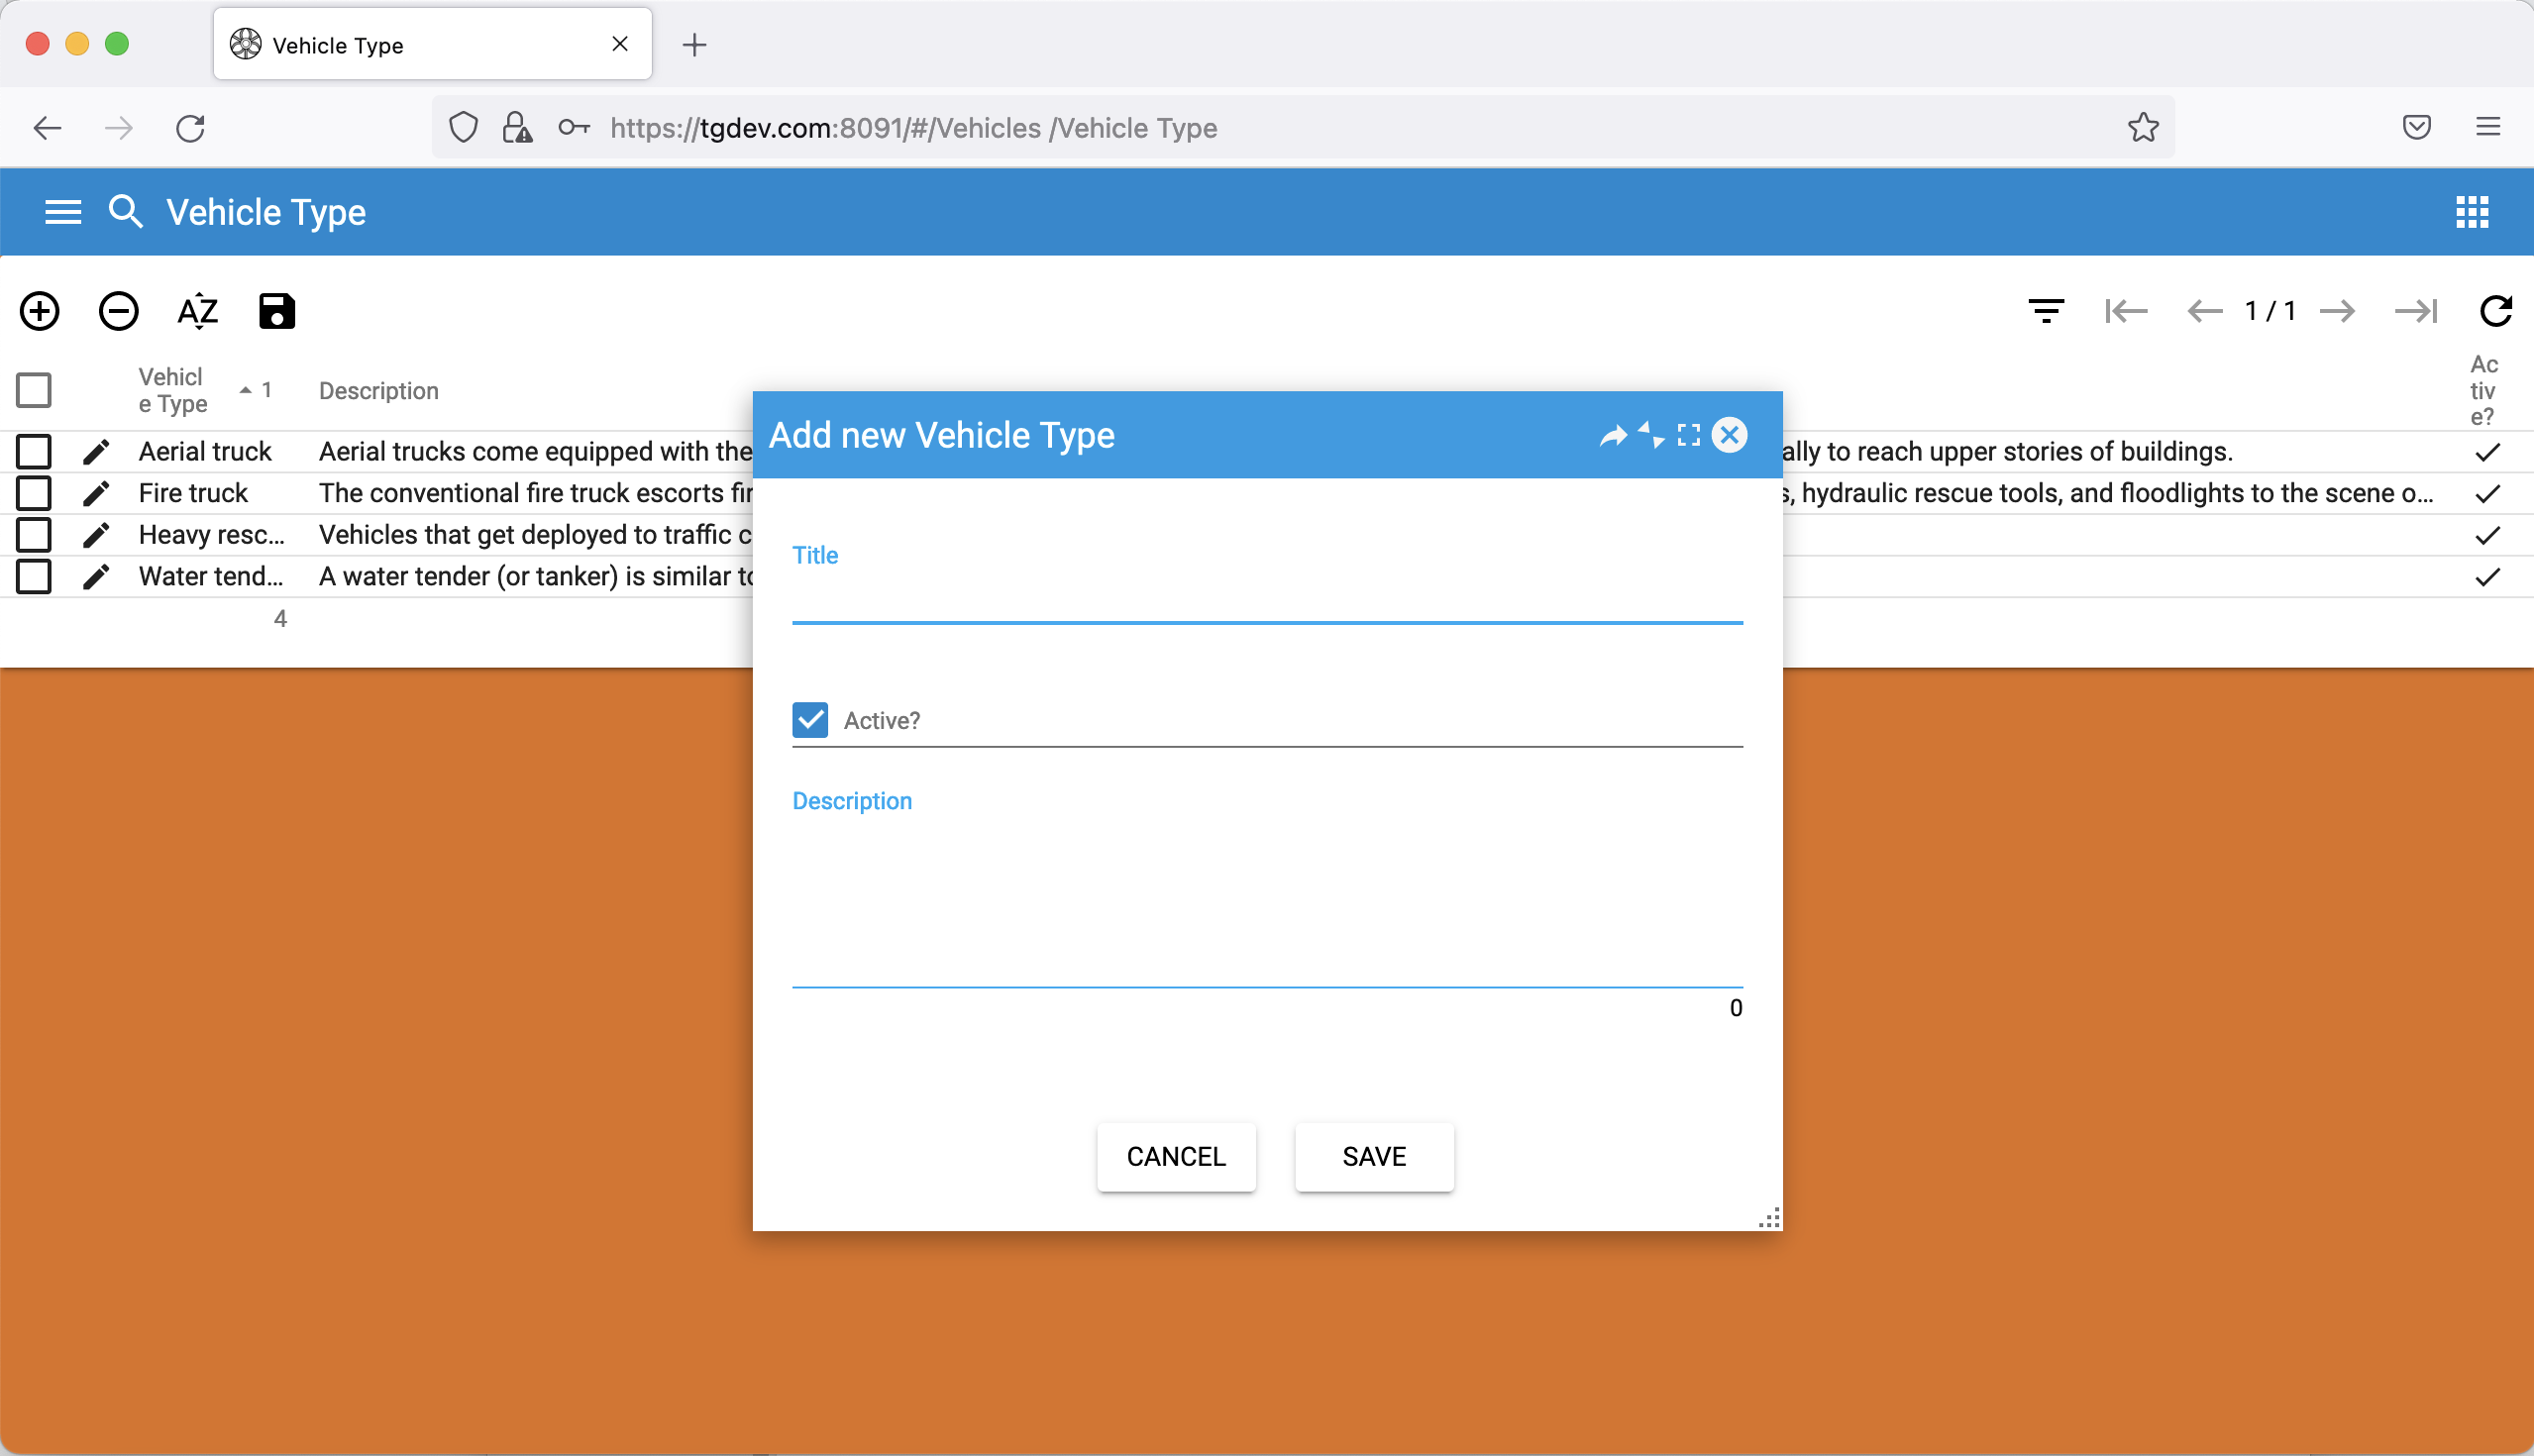
\includegraphics[width=0.95\linewidth]{sections/vehicles/images/20.png}
	\caption{Vehicle type creation.}\label{sections/vehicles/images/20}
	\end{figure}

\newpage
Users can search for existing vehicle types either by specifying title, which is auto-completed, or activity status, or description or all of them as displayed on
\hyperref[sections/vehicles/images/21]{Fig.~\ref*{sections/vehicles/images/21}}.

    \begin{figure}[!htbp]
	\centering
	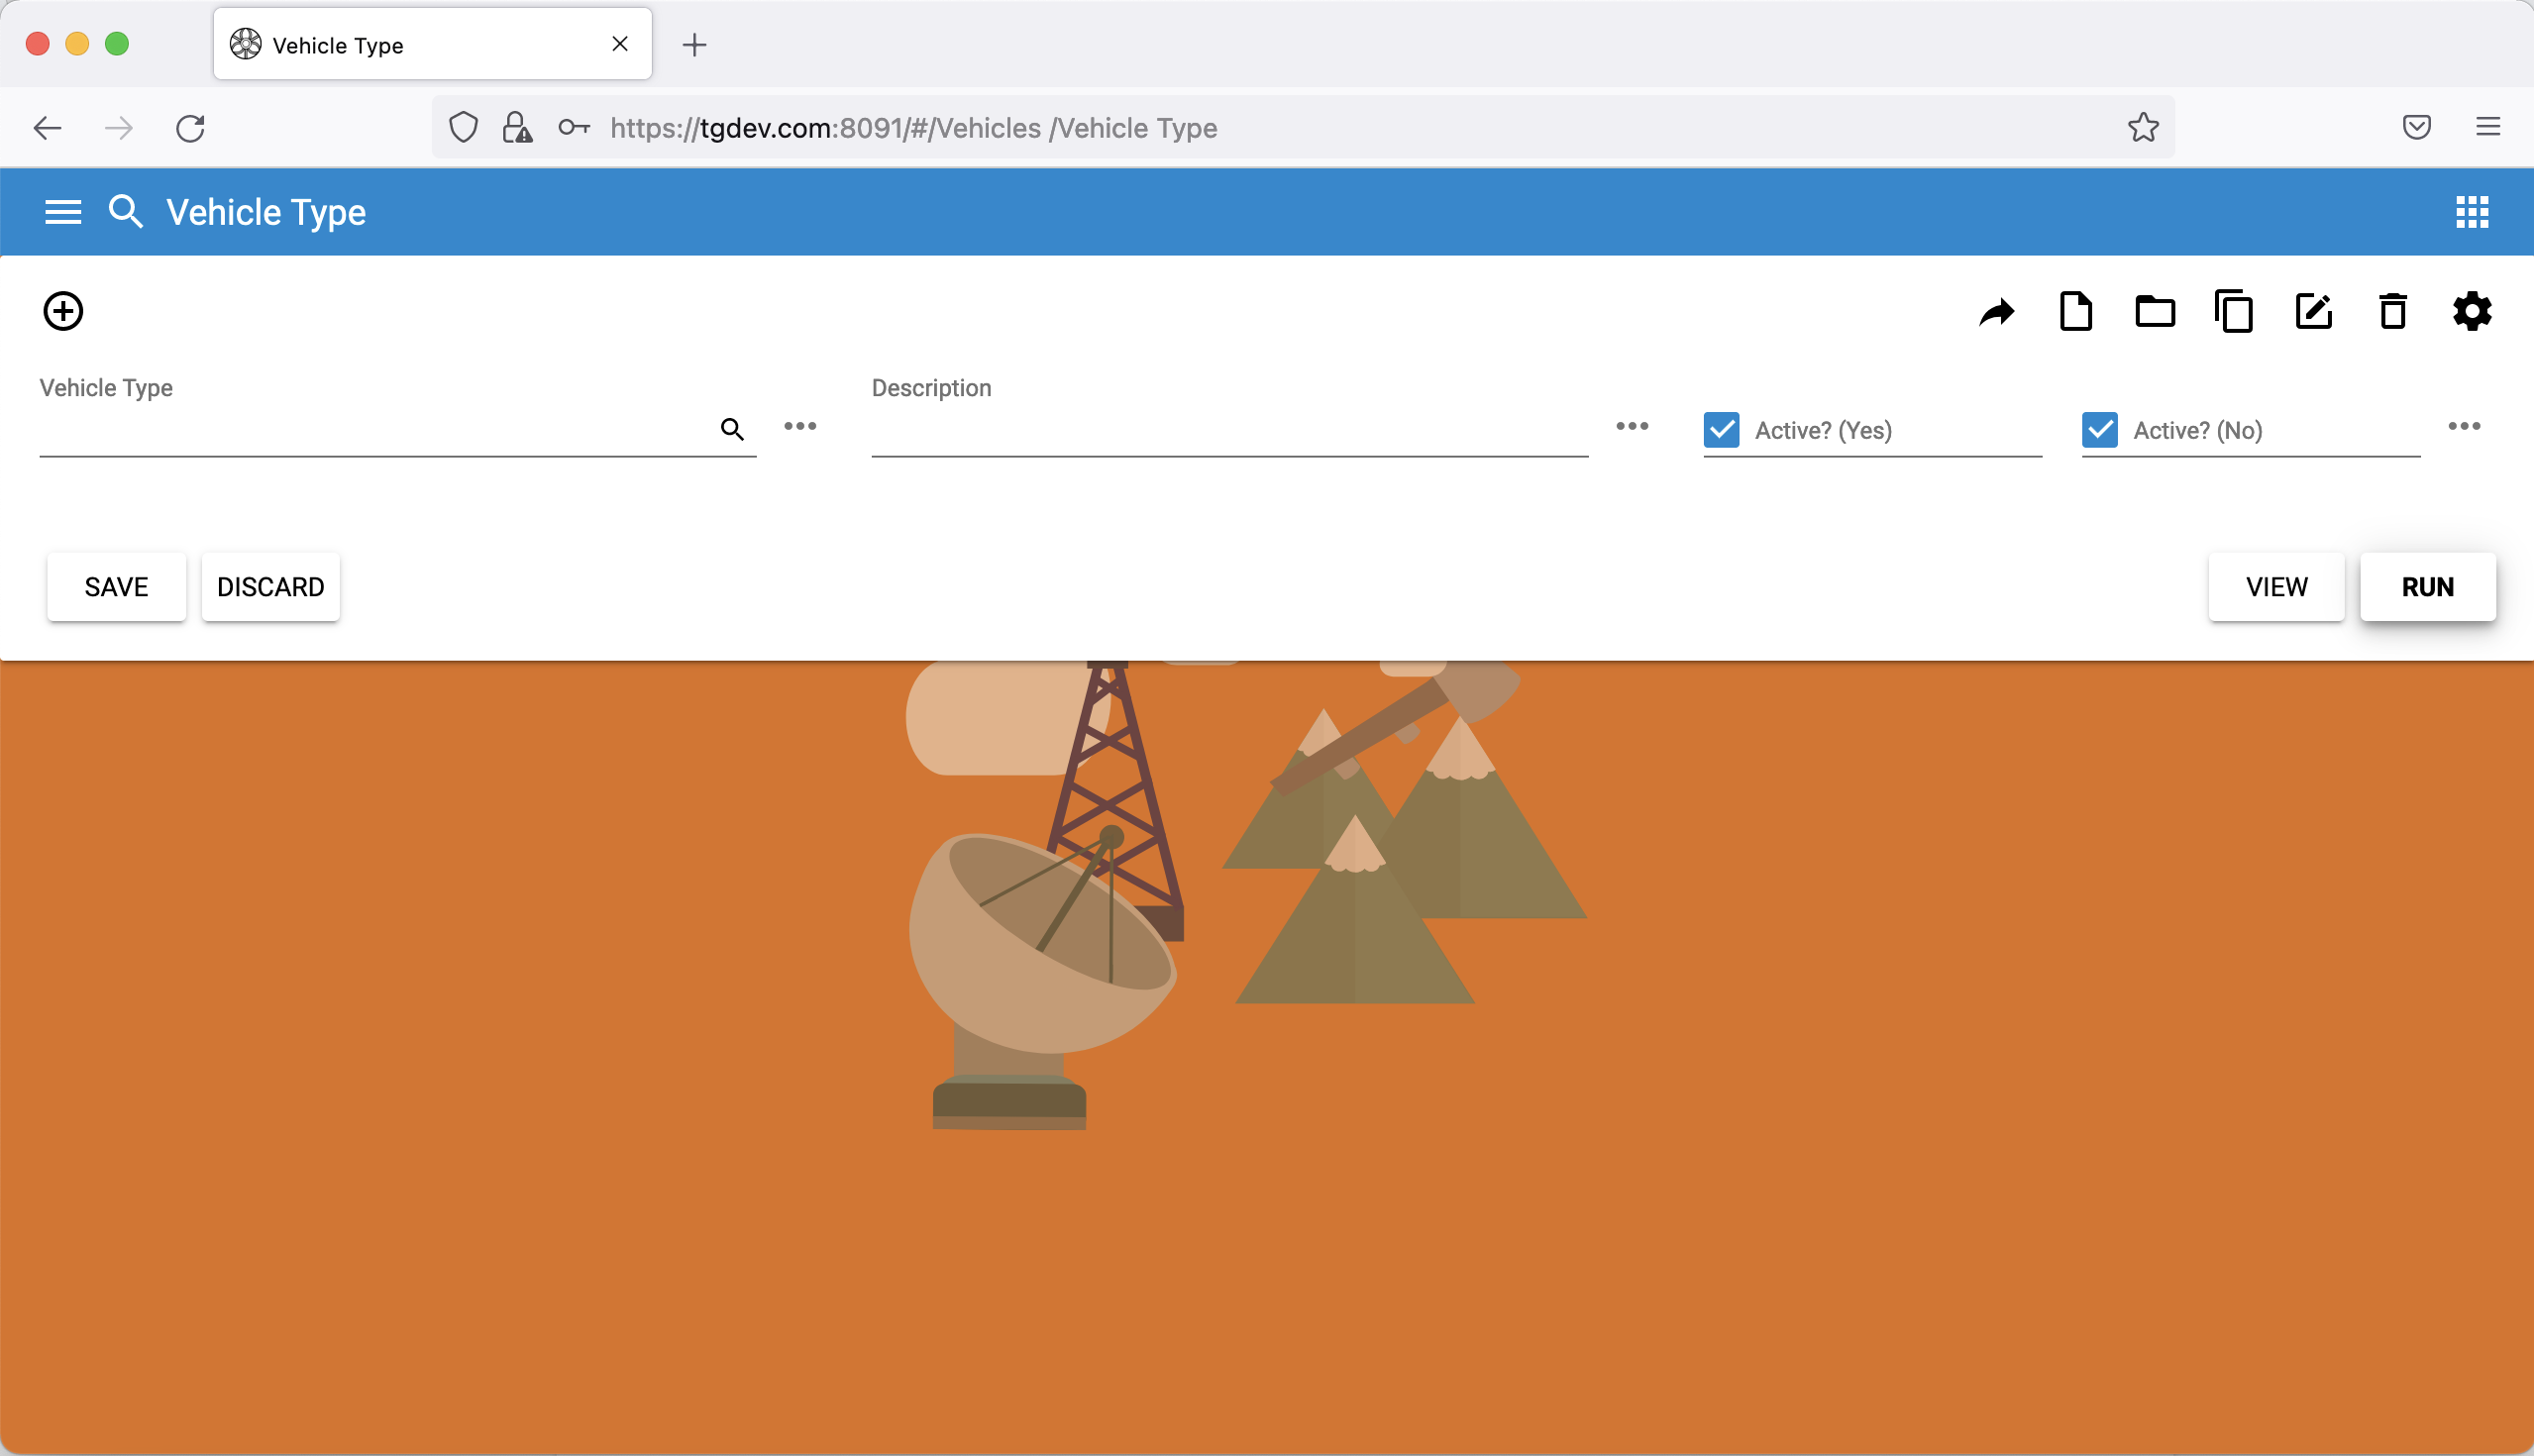
\includegraphics[width=0.95\linewidth]{sections/vehicles/images/21.png}
	\caption{Vehicle type search query.}\label{sections/vehicles/images/21}
	\end{figure}
	
\newpage
Search results are displayed along with title, activity status and description of the relevant vehicle types, as displayed on \hyperref[sections/vehicles/images/22]{Fig.~\ref*{sections/vehicles/images/22}}.

    \begin{figure}[!htbp]
	\centering
	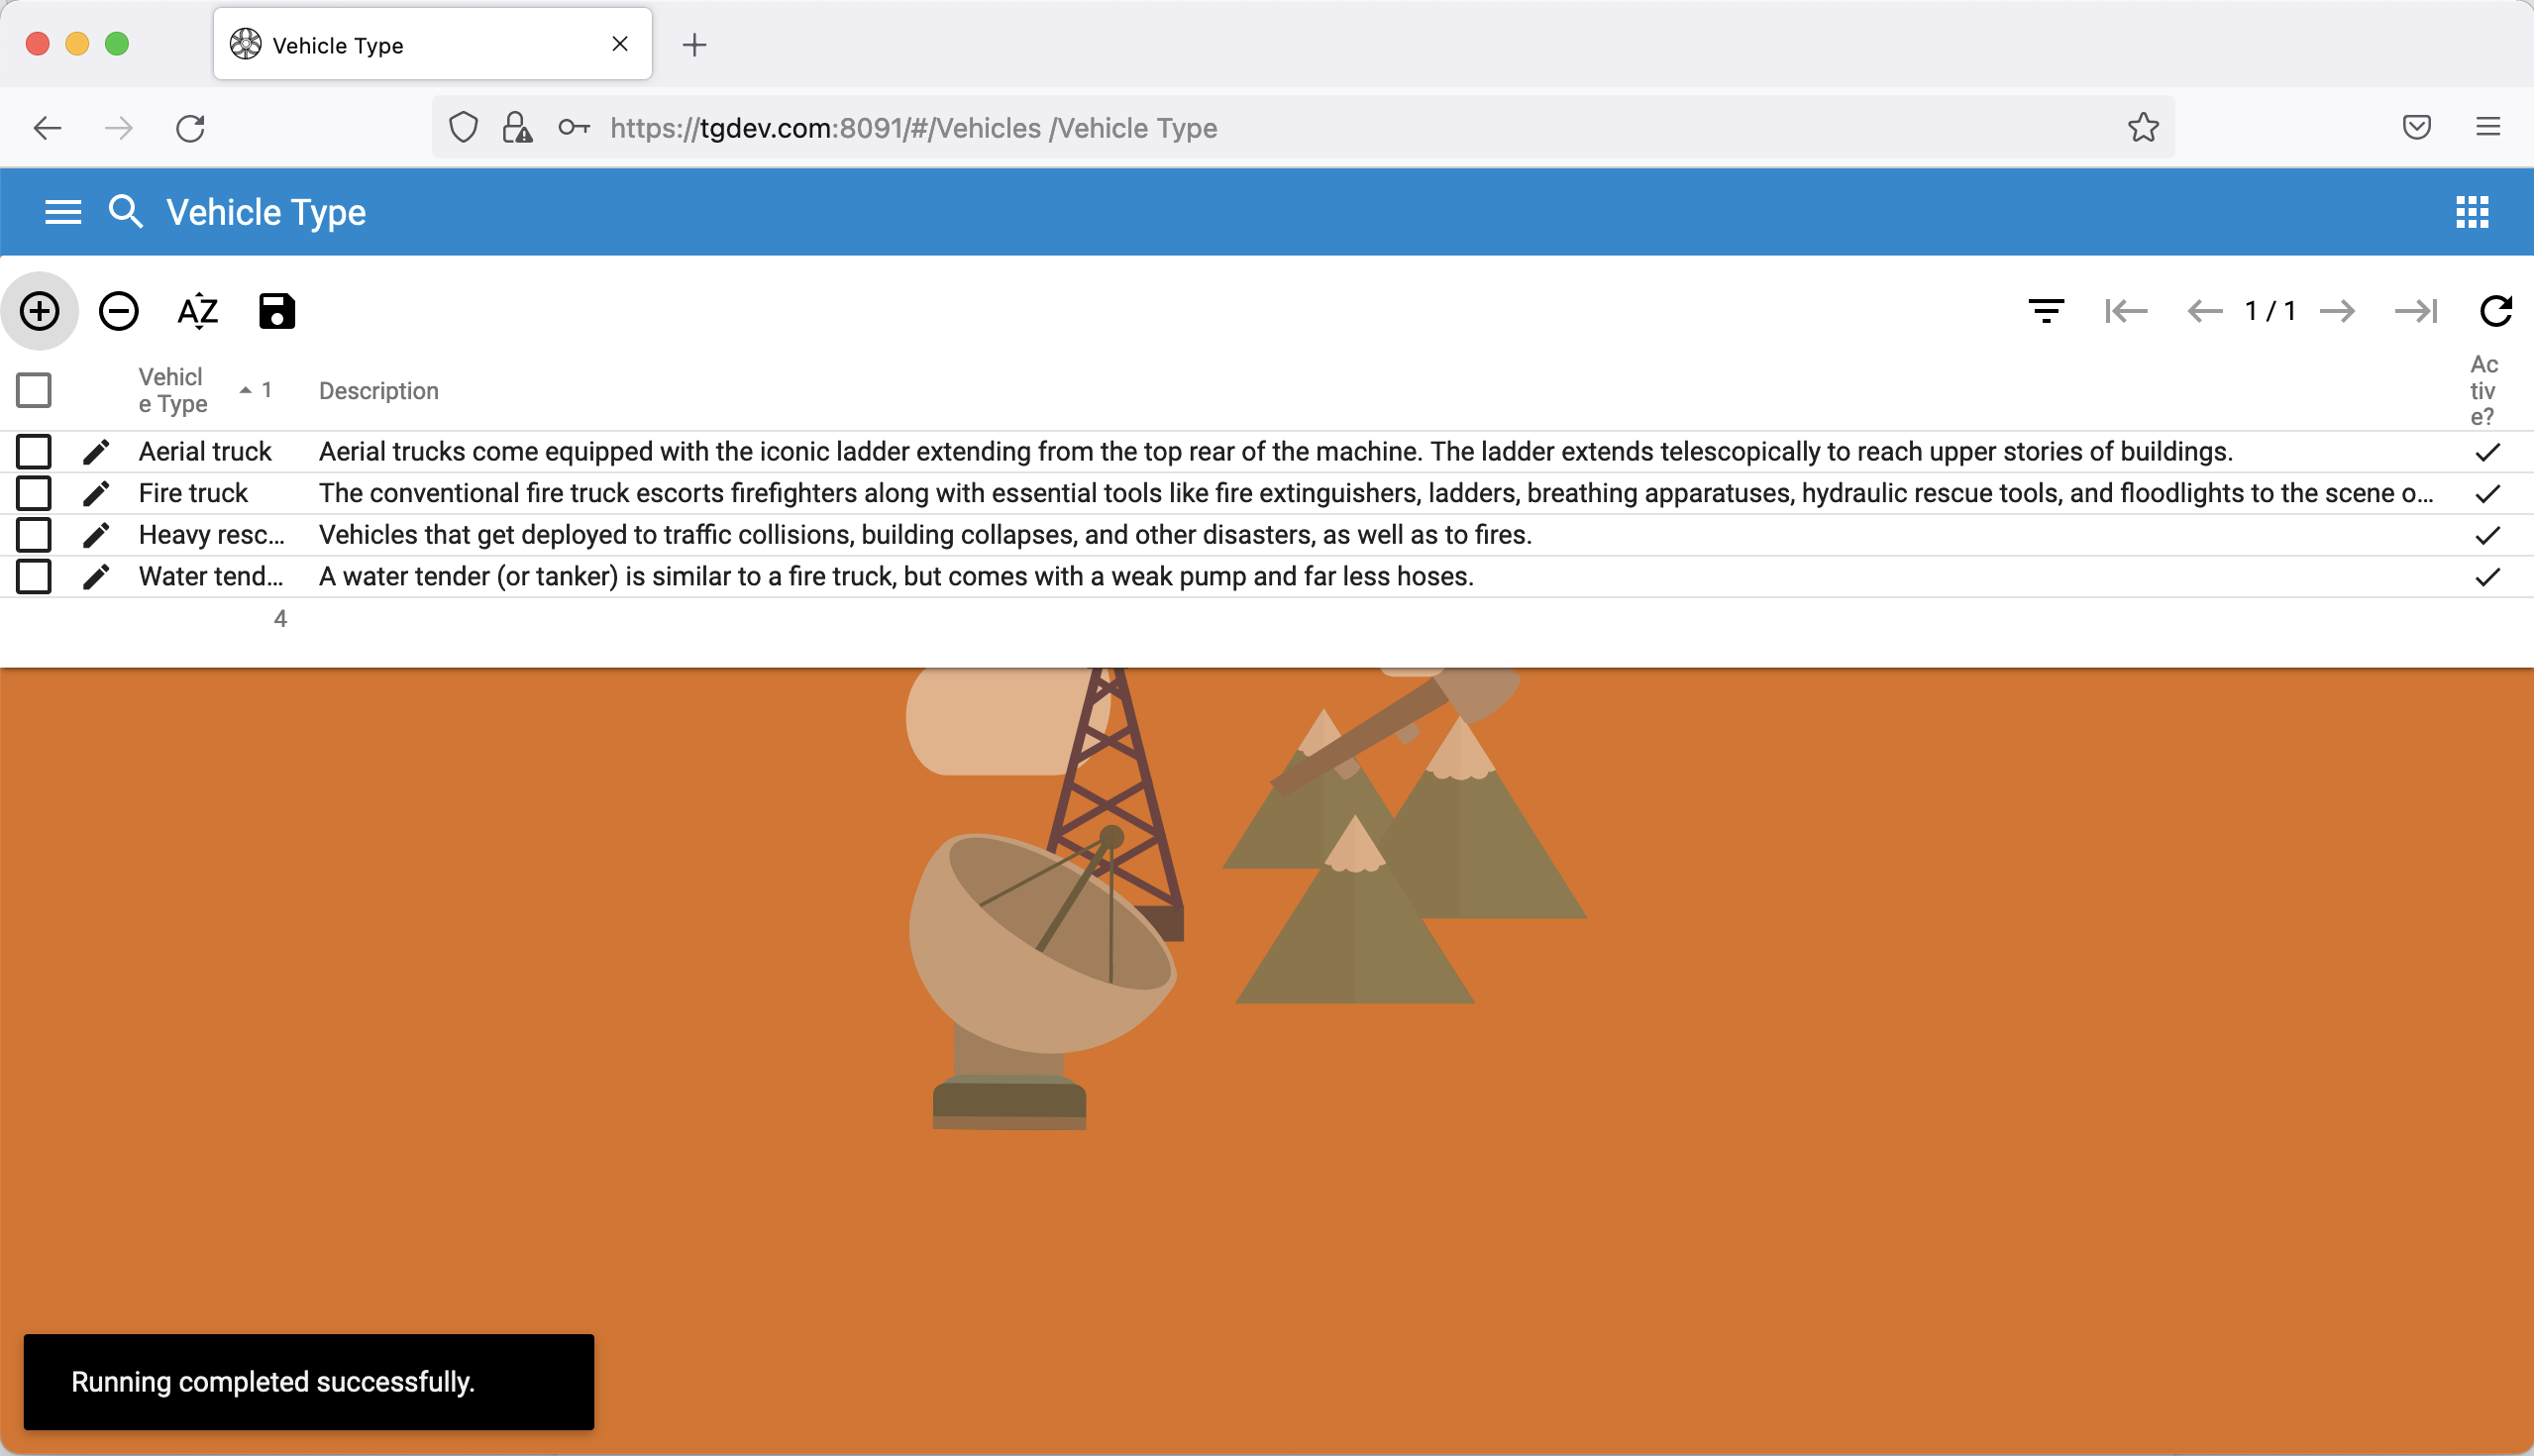
\includegraphics[width=0.95\linewidth]{sections/vehicles/images/22.png}
	\caption{Vehicle type search results.}\label{sections/vehicles/images/22}
	\end{figure}

\newpage
Users can edit existing vehicle types. On the main tab, as displayed on \hyperref[sections/vehicles/images/23]{Fig.~\ref*{sections/vehicles/images/23}}, users can edit title, activity status and description of the specific vehicle type.


    \begin{figure}[!htbp]
	\centering
	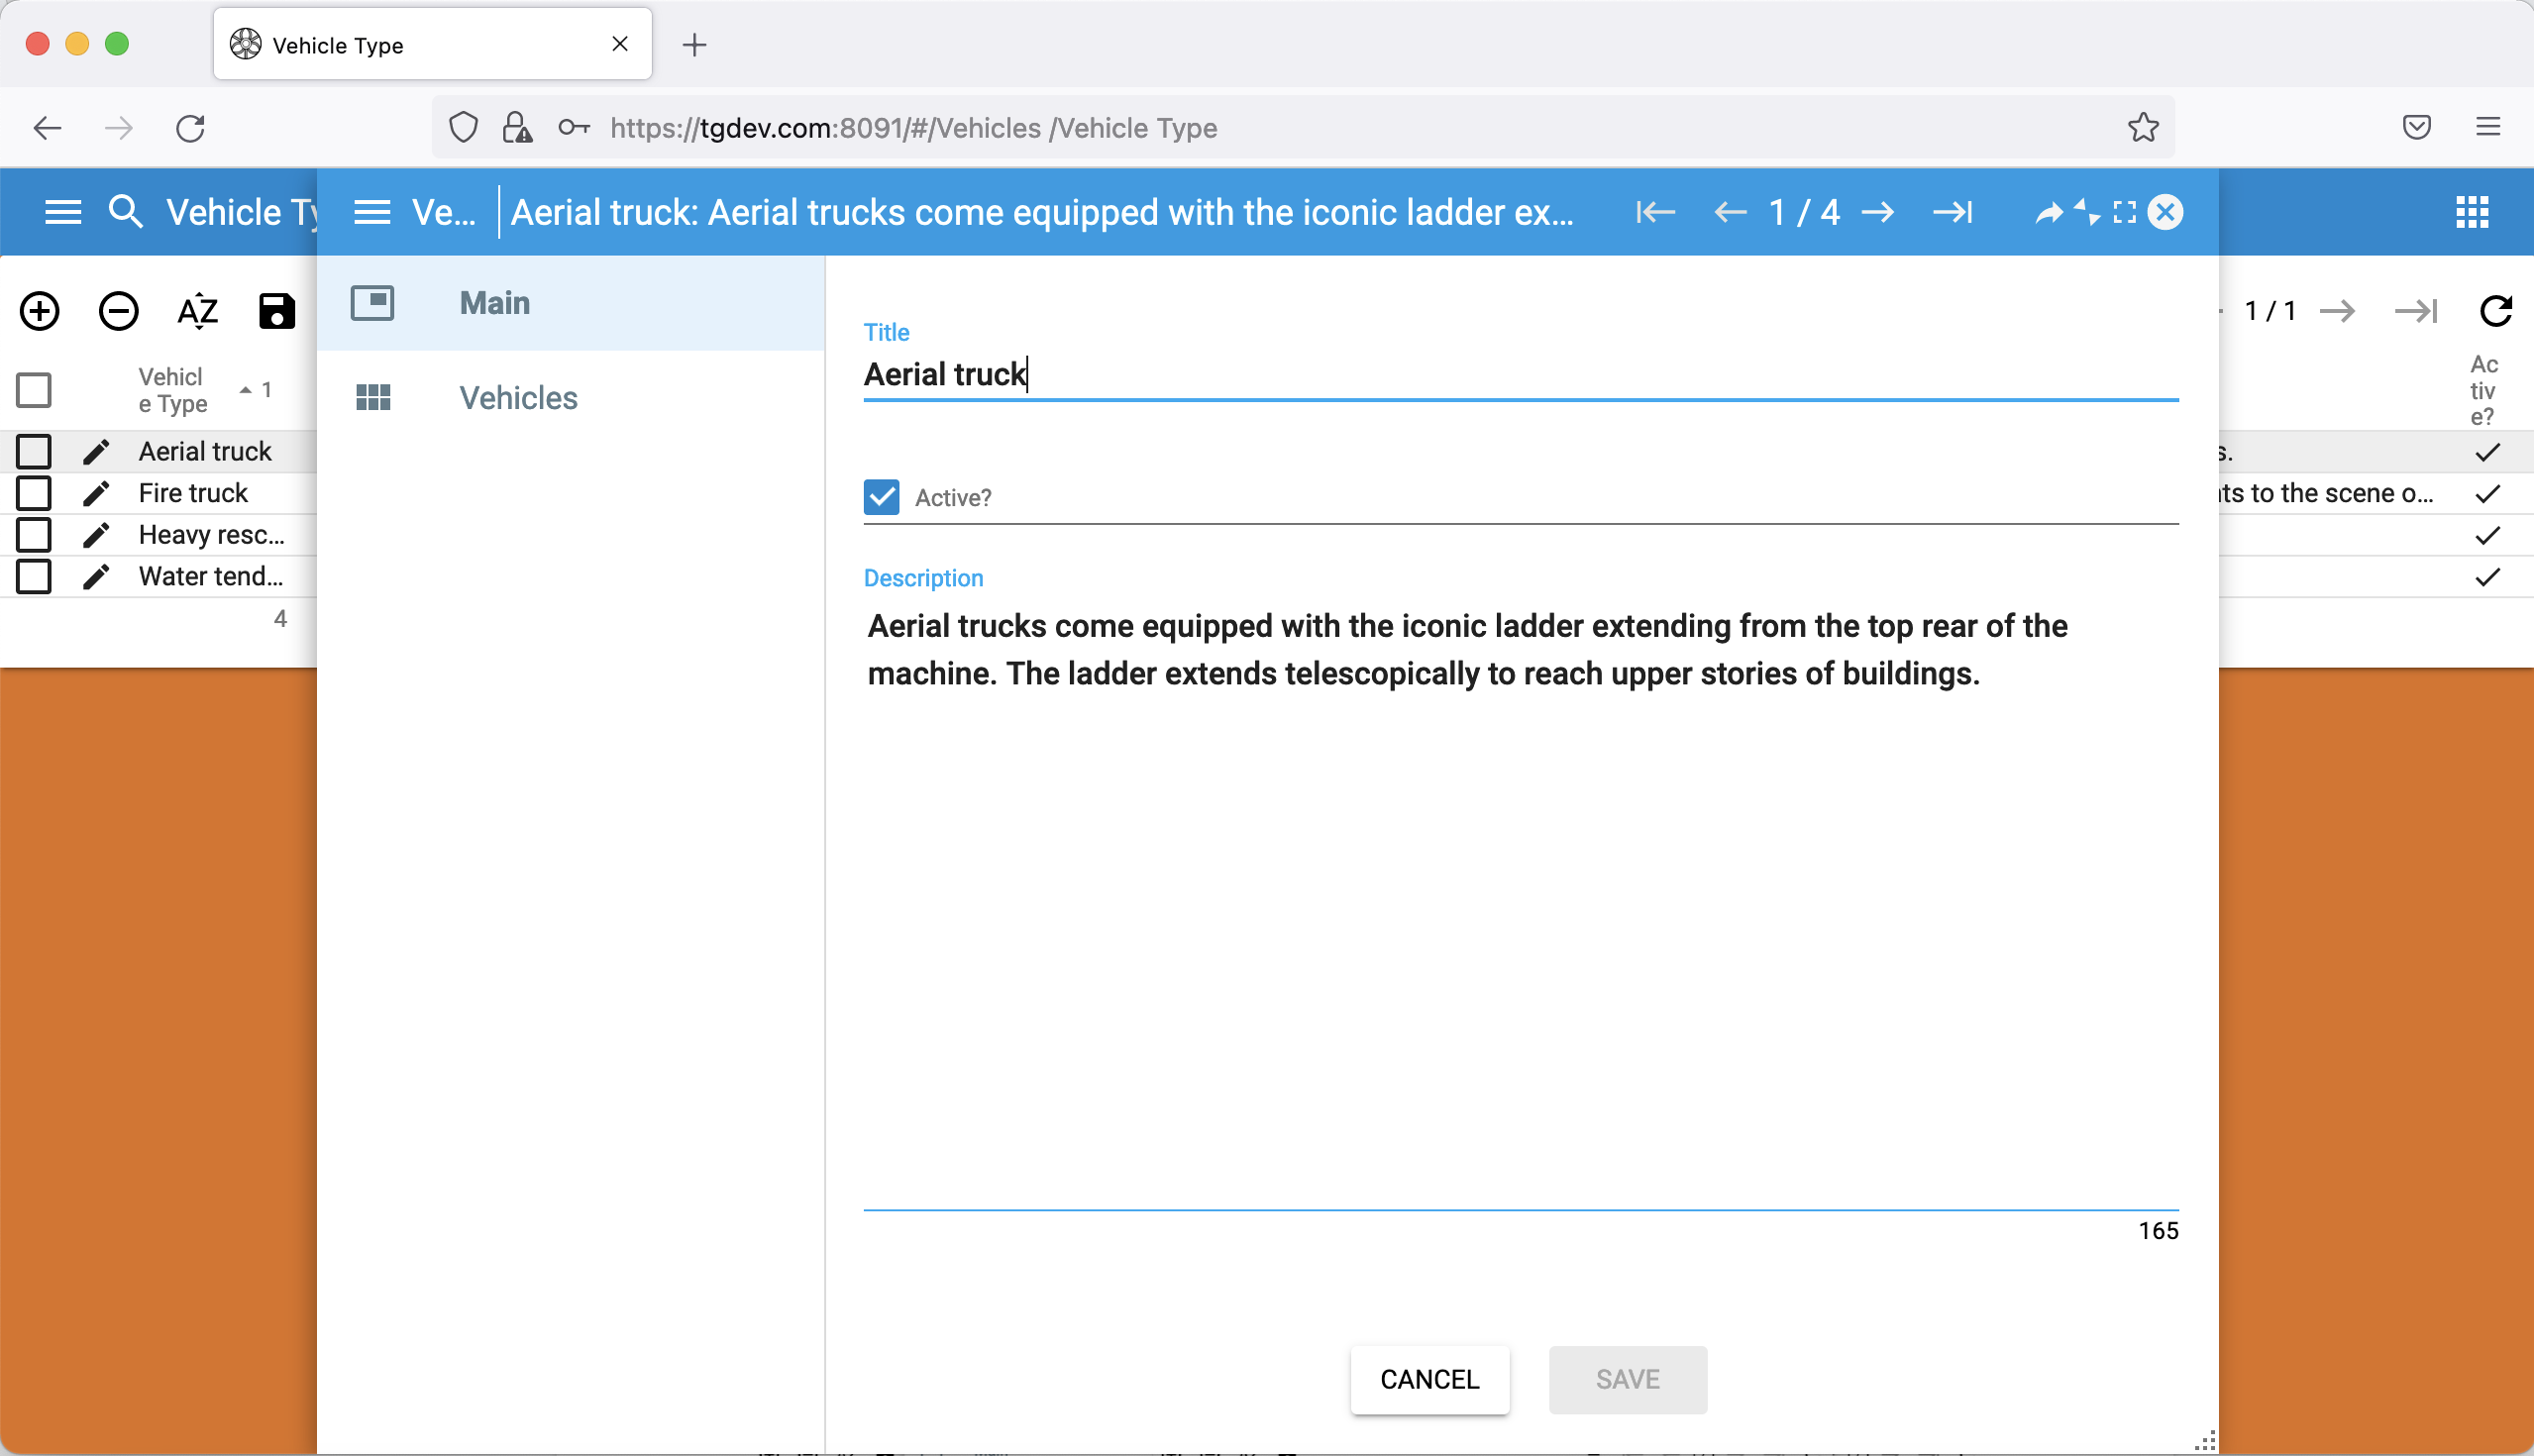
\includegraphics[width=0.95\linewidth]{sections/vehicles/images/23.png}
	\caption{Vehicle type editing.}\label{sections/vehicles/images/23}
	\end{figure}
	
\newpage	
On the ‘Vehicles’ tab, users can observe all of the vehicles related only to this specific vehicle type along with number, activity status, model, assigned driver, and description, as displayed on \hyperref[sections/vehicles/images/24]{Fig.~\ref*{sections/vehicles/images/24}}.

    \begin{figure}[!htbp]
	\centering
	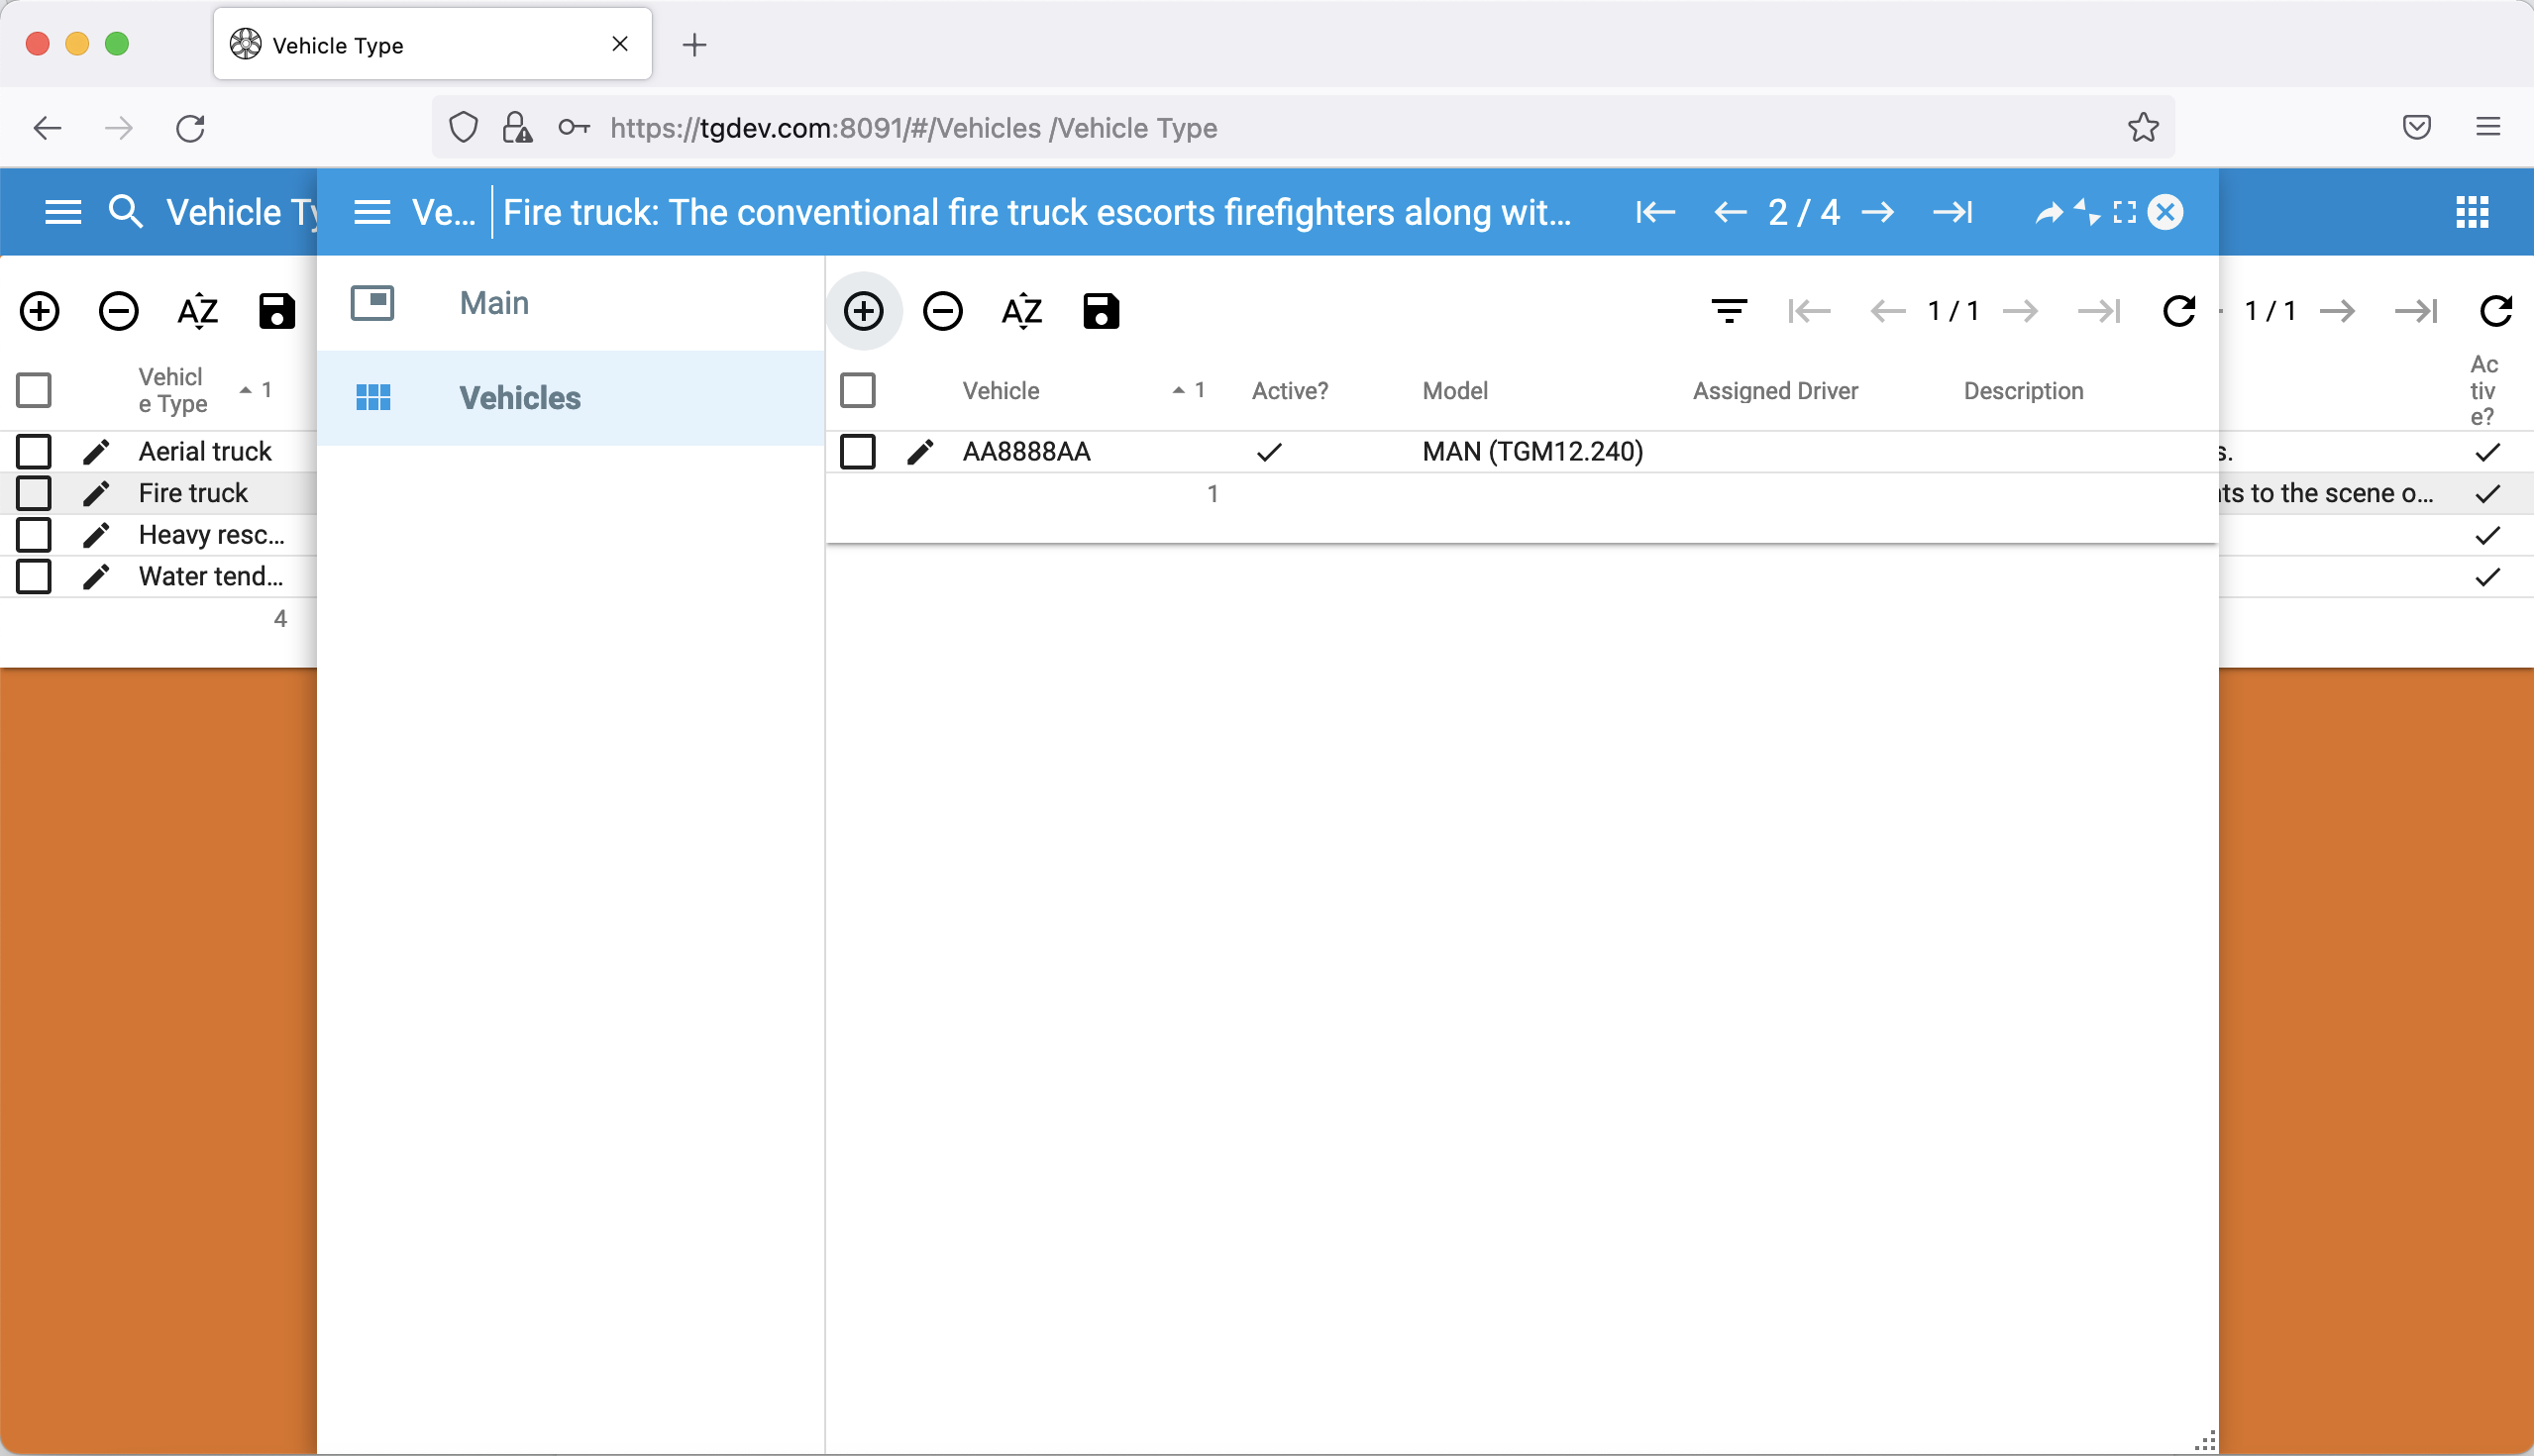
\includegraphics[width=0.95\linewidth]{sections/vehicles/images/24.png}
	\caption{Embedded vehicle search results.}\label{sections/vehicles/images/24}
	\end{figure}

\newpage
Users can also search for existing vehicles related only to this specific vehicle type either by specifying number, which is auto-completed, or activity status, or model, or assigned driver, or description, as displayed on
\hyperref[sections/vehicles/images/25]{Fig.~\ref*{sections/vehicles/images/25}}.

    \begin{figure}[!htbp]
	\centering
	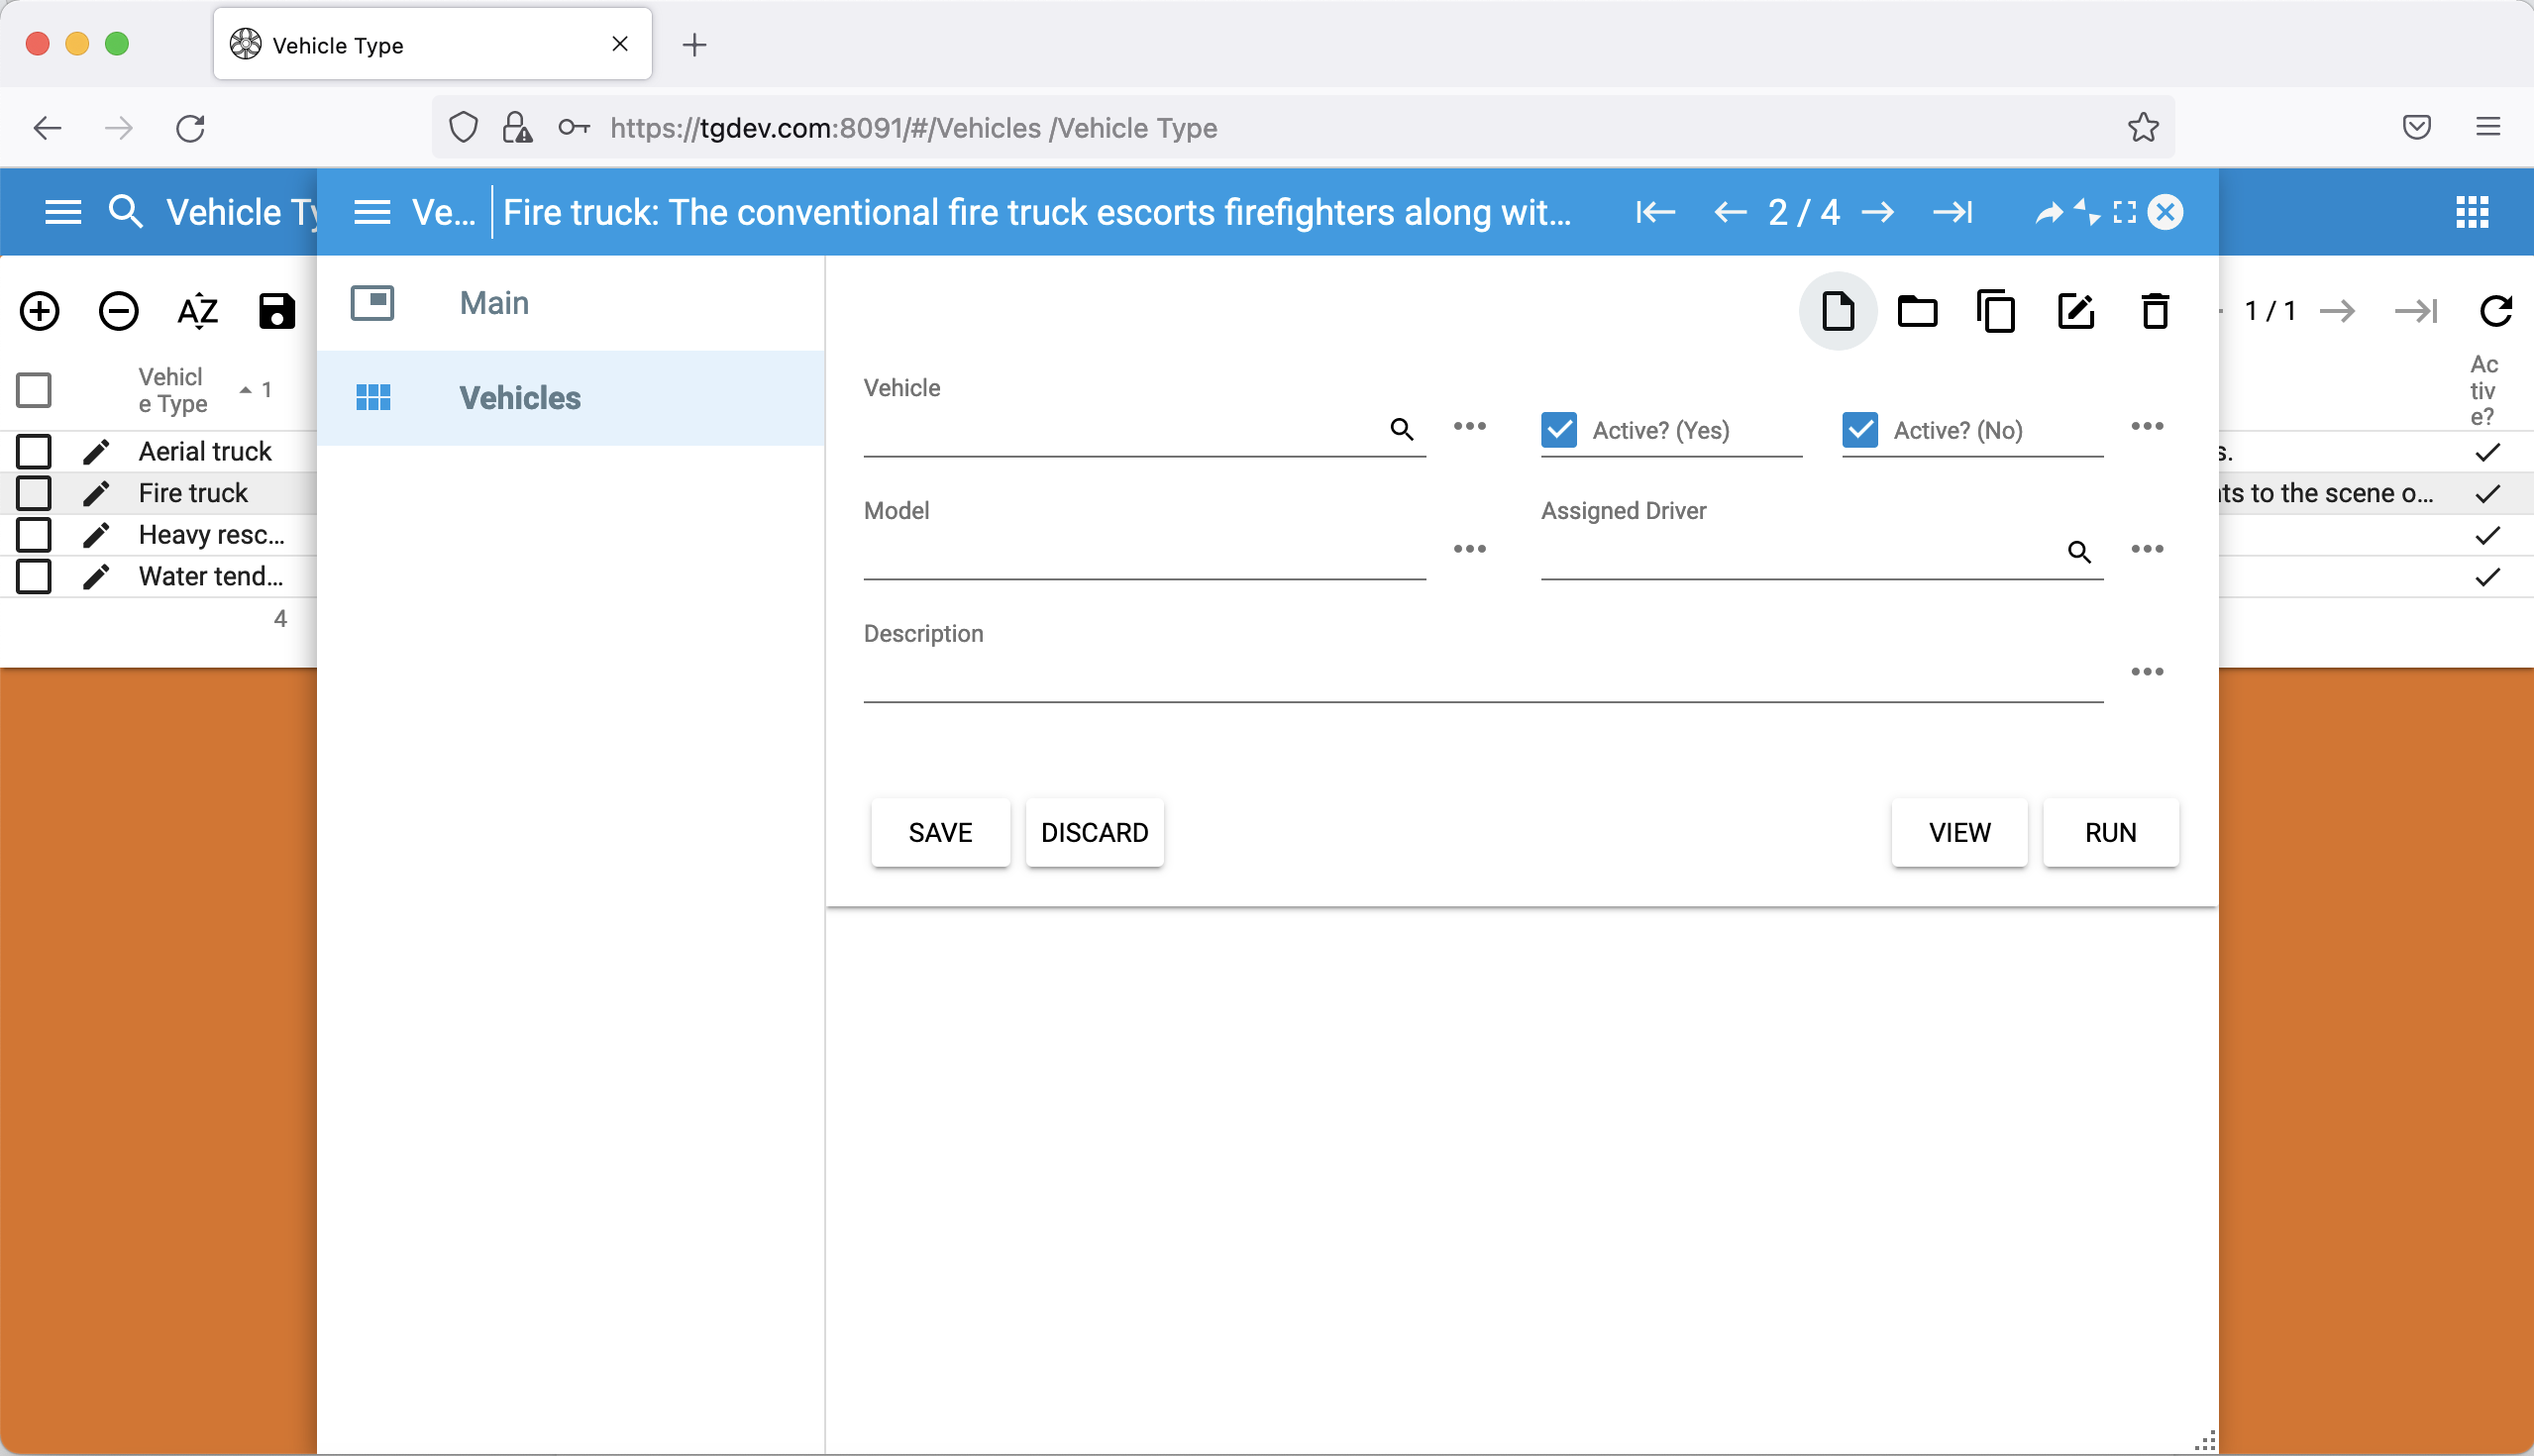
\includegraphics[width=0.95\linewidth]{sections/vehicles/images/25.png}
	\caption{Embedded vehicle search query.}\label{sections/vehicles/images/25}
	\end{figure}
	
\newpage
Users can also create a new vehicle by filling in its number in format AA9999AA and activity status, as well as its model, assigned driver (optional), and description (optional) as displayed on \hyperref[sections/vehicles/images/26]{Fig.~\ref*{sections/vehicles/images/26}}. Vehicle Type field is automatically auto-completed with this specific vehicle type.

    \begin{figure}[!htbp]
	\centering
	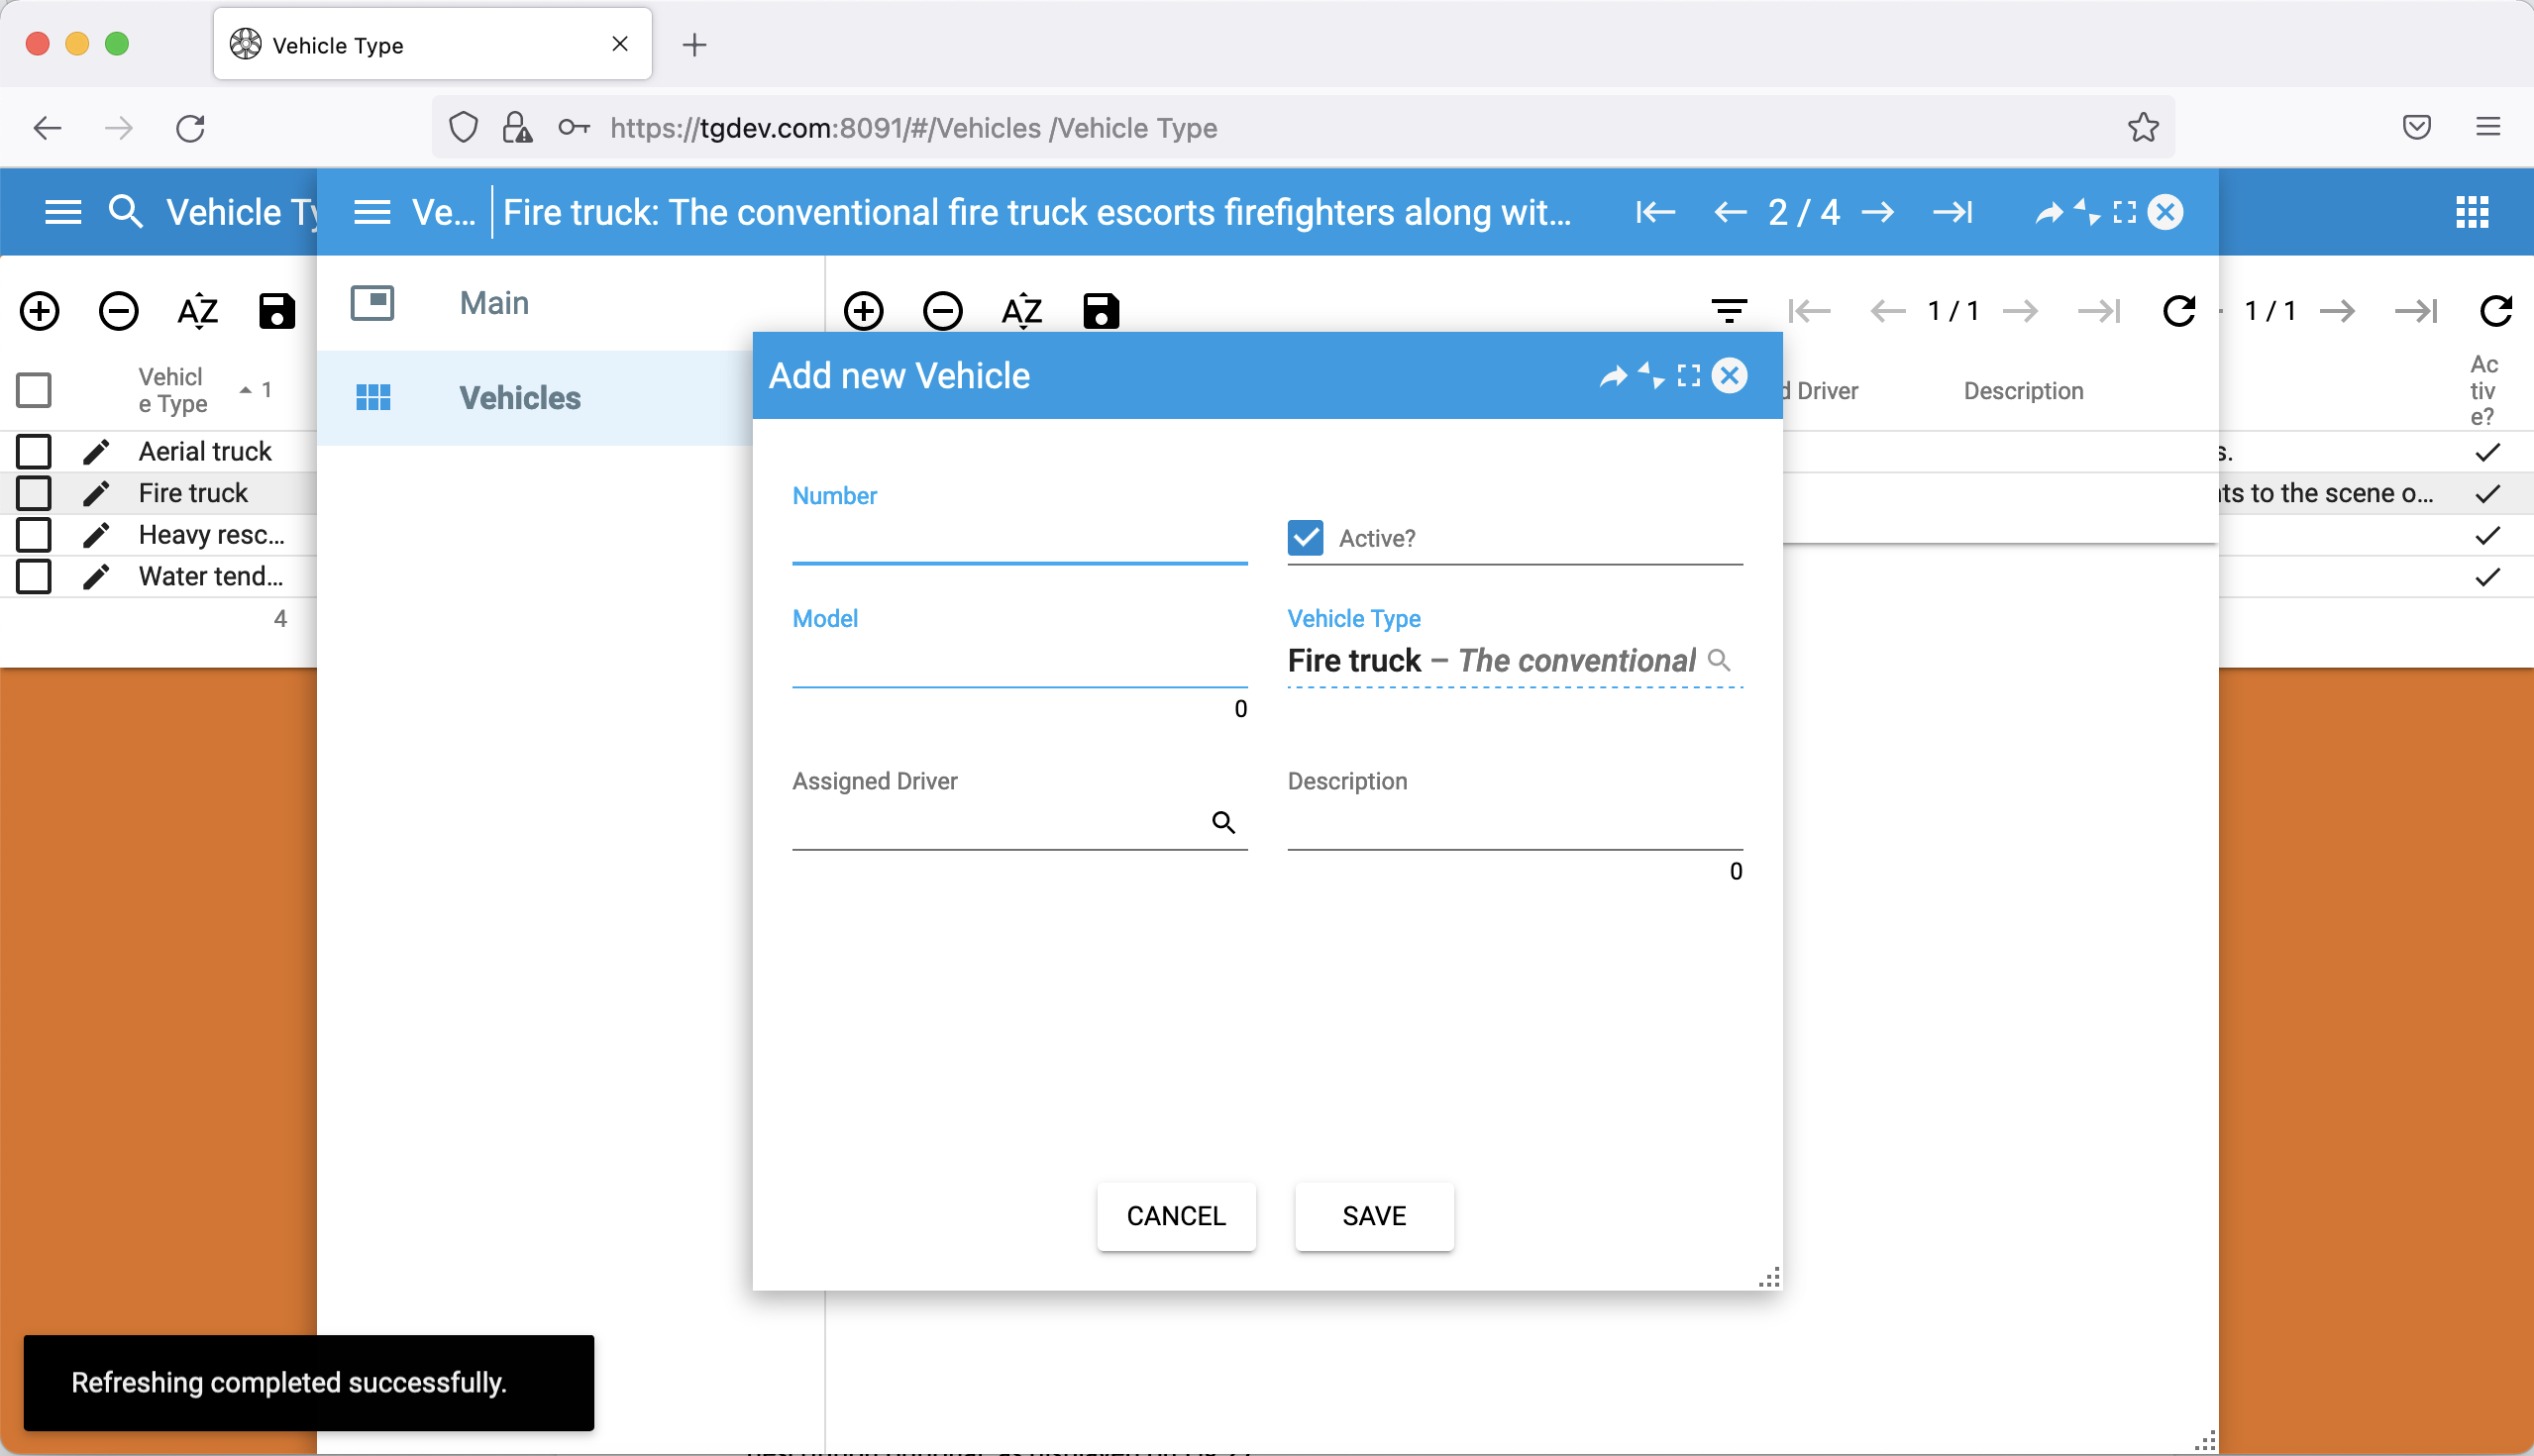
\includegraphics[width=0.95\linewidth]{sections/vehicles/images/26.png}
	\caption{Embedded vehicle creation.}\label{sections/vehicles/images/26}
	\end{figure}

\newpage	
\subsection{Vehicle}
In order to perform registration, classification and tracking of vehicles correctly, users can create vehicles. When creating a new vehicle, users have to fill in its number in format AA9999AA, activity status, corresponding vehicle type which is auto-completed, model, assigned driver (optional), and its description optional, as displayed on \hyperref[sections/vehicles/images/27]{Fig.~\ref*{sections/vehicles/images/27}}.

    \begin{figure}[!htbp]
	\centering
	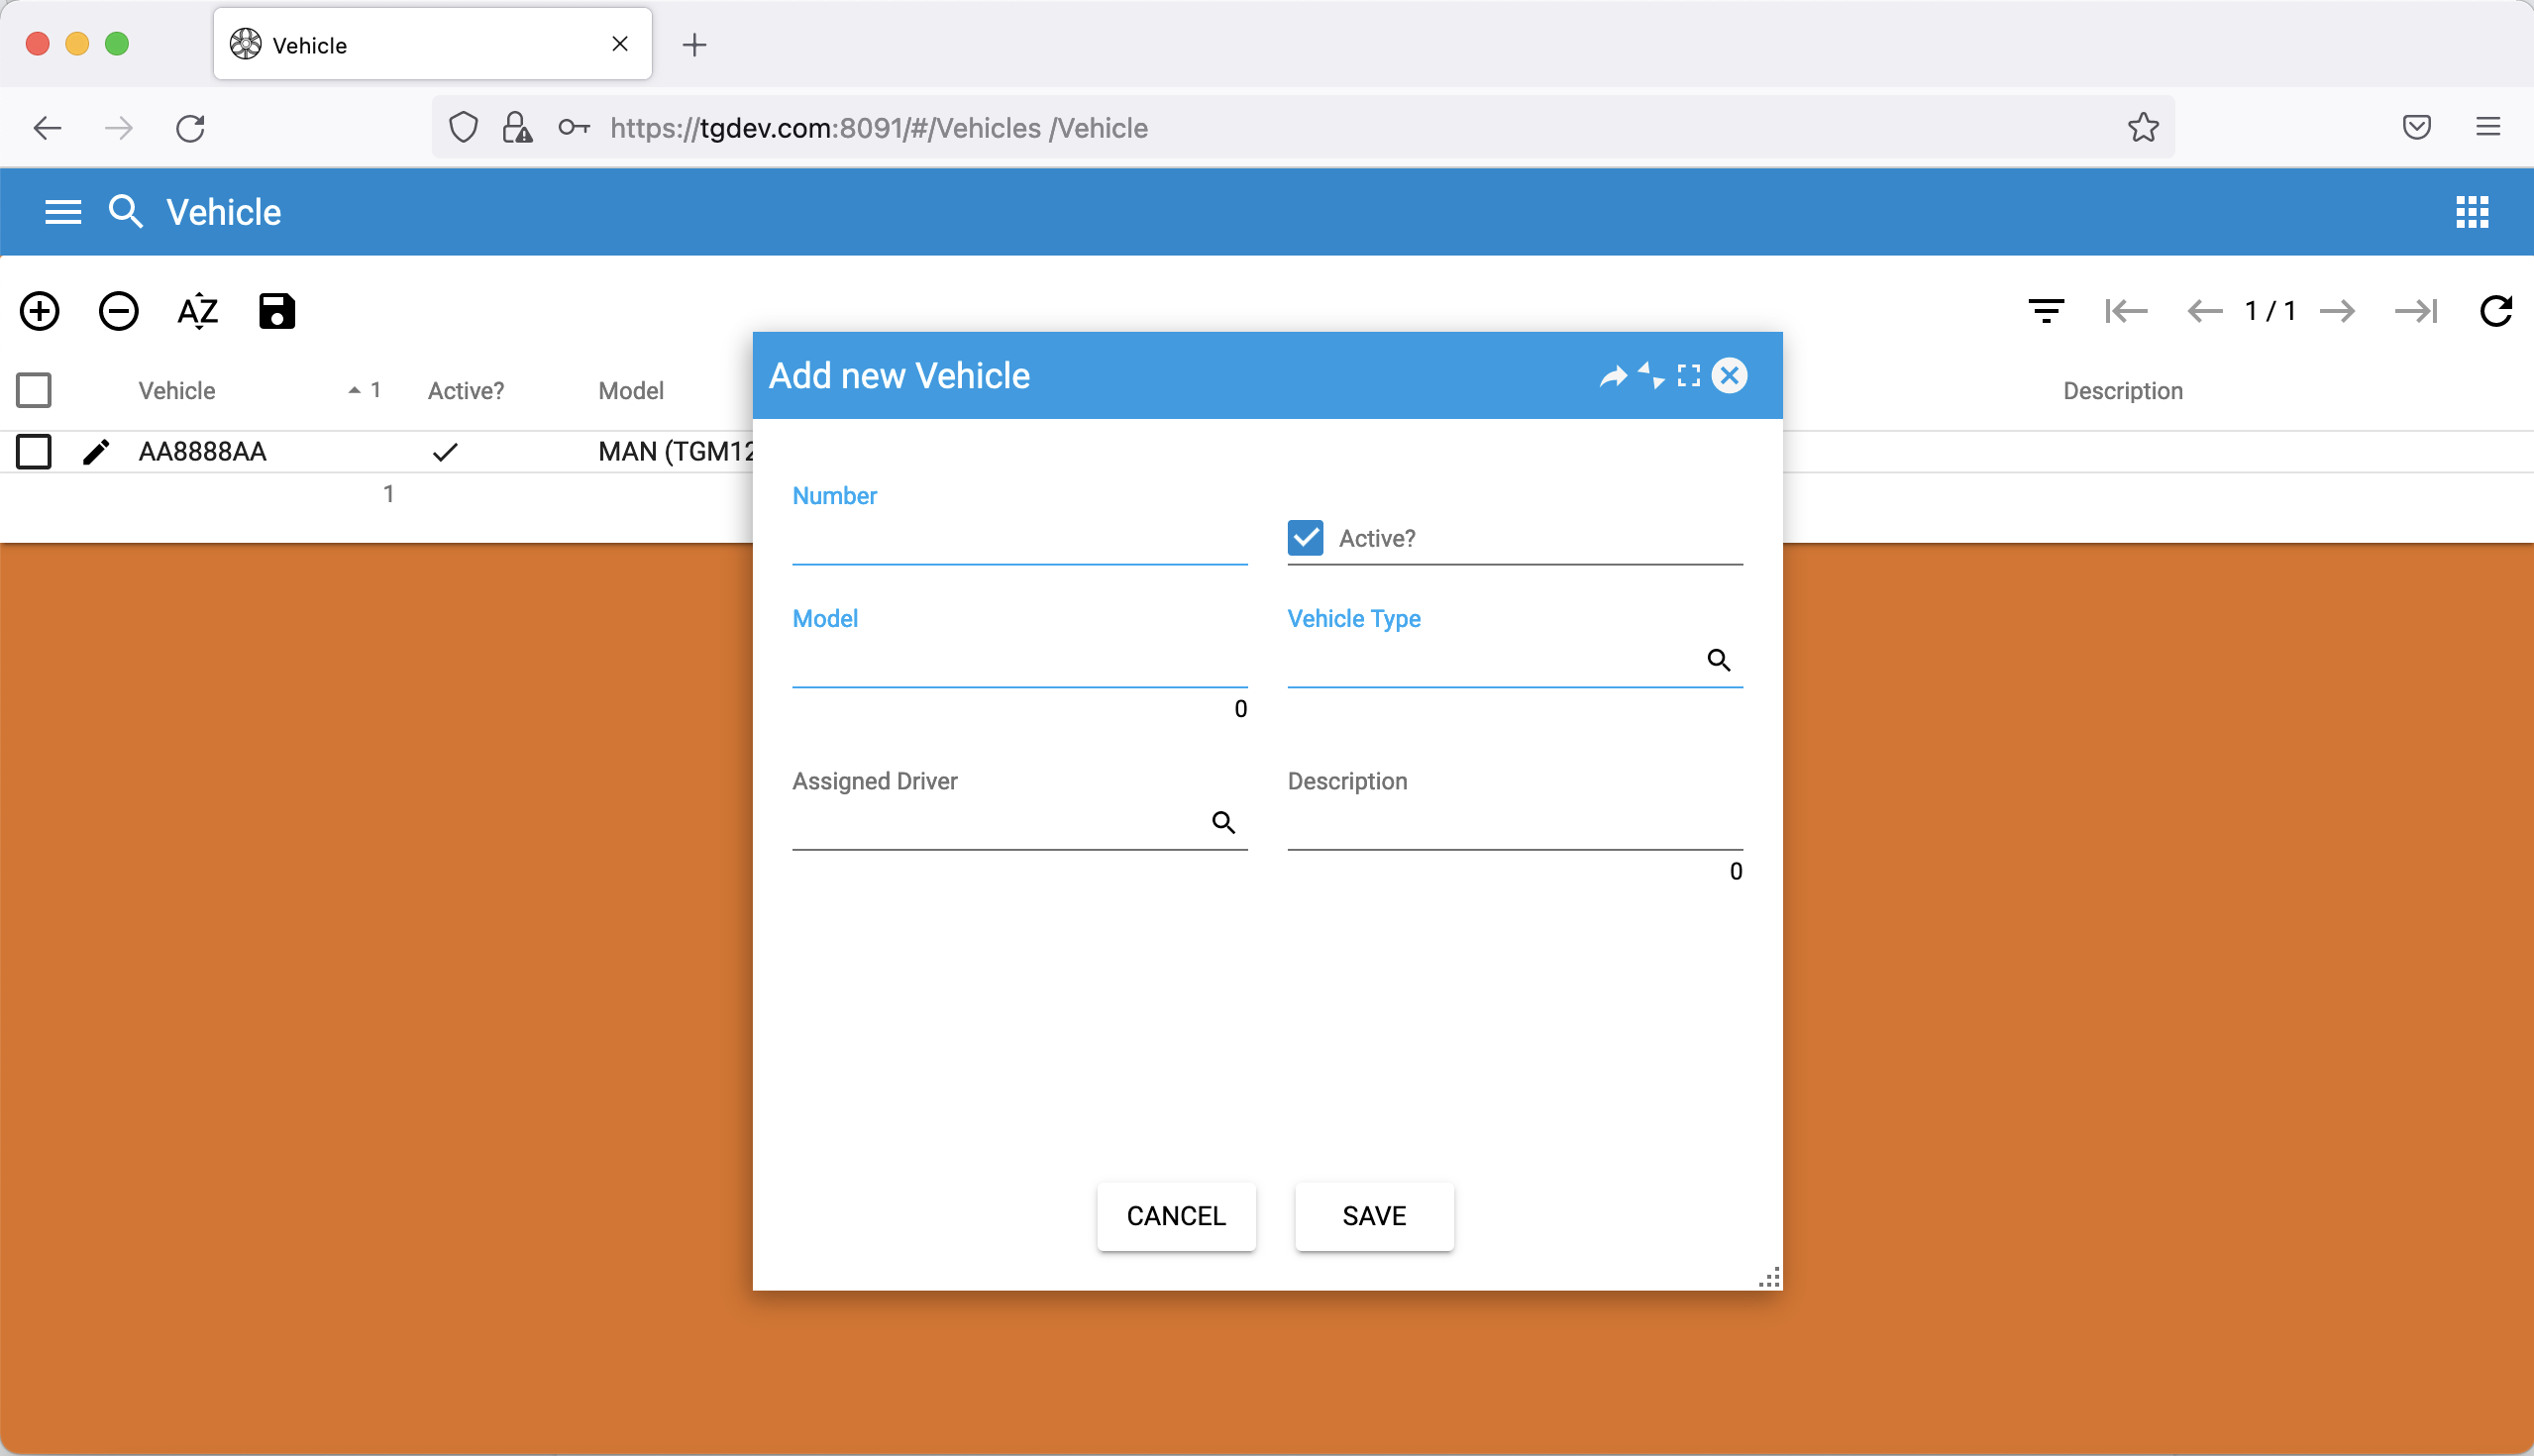
\includegraphics[width=0.95\linewidth]{sections/vehicles/images/27.png}
	\caption{Vehicle creation.}\label{sections/vehicles/images/27}
	\end{figure}

Users can also search for specific vehicles and edit them as described in the vehicle type embedded master section.